%ब
\chapter{Results and Discussions}
\section{Introduction}
Performance of database systems is commonly measured in terms of the
\textit{Response time} and \textit{Throughput}(\todo{cite Demurjian, Berkely}).
Response time refers to the time  a database system takes to process an
operation and produce results to the end user . Measuring response time for a
database operation is similar to a black-box evaluation because it is measured
without considering the internal functioning  of the database system. According
to (\todo{cite Demurjian}) such an evaluation is ideal for a complete database
system to measure its performance and to give the users details about its
efficiency and speed in performing operations. In this thesis, response time and
throughput are the measures used to gauge the performance of Cassandra while
referential integrity validation is implemented using the \ac{API}.

Response time for each  operation that triggers  a referential integrity
validation from all the solutions are measured during the experiments.
% This included the time involved to access and retrieve metadata for the entities
% and also the time for validating referential integrity by the
% \texttt{ValidationHandler}. 
The response time of Cassandra when such validations
are not in place is also measured and considered as a baseline with which to
analyse the solutions. Such a comparison determines the degree of change in
speed of Cassandra when such overheads are introduced and gives users useful
information about how each solution affects the performance of the database
system.

The second performance measure used is \textit{Throughput} and in the
experiments, it is measured as operations per second for  the operations
triggering referential integrity validation namely, \texttt{Create},
\texttt{Update} and \texttt{Delete}.
% A single operation
% stands for each time an entity is inserted, updated or deleted. Note that only
% the operations that introduce the referential integrity validation in Cassandra
% is measured and thus \texttt{read} operations are not measured in terms of
% response time or throughput.

% It has to be noted that the operations are prone to  external factors like
% network latency, bandwidth, network routing, network workload among others which
% typically affect a network consisting of several machines and users. This is
% because the Cassandra cluster used in the experiments is deployed over a
% network that is used by many users concurrently thus exposing the operations to
% such factors. Identifying such factors and analysing them is beyond the scope of
% this thesis and the analysis is strictly in terms of how the metadata storage
% and referential integrity validation affects Cassandra's performance.

 The results from the experiments were used to
analyse the performance of the four solutions  and this is discussed in the
following sections. 
Section~\ref{sr:baseline} presents the results for the
baseline experiment where the operations performed on the entities are just as
it would be performed in Cassandra without any referential integrity validations
or constraint metadata.
Section~\ref{sr:insert} analyses the results of all the solutions for the
\texttt{insert} operation.
Section~\ref{sr:update} presents the analysis for the \texttt{update} operation
for all the solutions.
Section~\ref{sr:delete} discusses the results of the solutions for the
\texttt{delete} operation.

\newcommand{\Width}{0.5\textwidth}
\newcommand{\TB}[1]{\textbf{#1}}

\section{Overview}
The experiments were run with the objective of measuring the performance of the
solutions and to determine how metadata storage affects the performance of the
operations. The results from these experiments are presented in
Tables~\ref{tres:ResponseTime} and~\ref{tres:Throughput}.

These results show that the solutions do not have the same performance as each
of them have different response times and throughput. This difference in the
performance is due to the different ways of storing the metadata. Recall that
Solutions~1 and 2 save metadata along with the entity where Solution~1 stores it
in every row and Solution~2 stores it in the top row of a column family. On the
other hand, Solutions~3 and 4 store metadata separate from the actual adata
where both solutions save it in a separate column family but Solution~4 stores
the metadata column family in a separate cluster. The way metadata is stored and
retrieved in each solution affects its performnce during validation, where
constraints are retrived and used.

The results show that Solution~4 takes the least time to execute an operation on
an entity, which means that it is faster than the other solutions to perform the
\ac{CRUD} operations on the entitites.This is because this solution caches the
metadata for an entity and avoids connecting to the external cluster or column
family each time an operation is invoked. Solutions~1, 2 have
approximately similar response times since metadata is a part of the entity and
accessing it requires no additional connections to another column family.
Solution~1 performs marginally better than Solution~2 and this is because
Solution~2 has an additional search operation ot identify the top row in a
column family to locate the metadata.
% their metadata access for
% these solutions are easier as metadata is a part of the entity and no additional
% connection to a metadata column family is required.
Solution~3 takes slightly longer than the rest of the solutions and this is
because 
% of the way
% the metadata is accessed for the entities in this solution.
% % irrespective of whether an entity is a parent or child the %
% \texttt{ValidationHandler} performs the same check the metedata of the entity
% % for all the solutions. It is when this check is made it is clear if the
% entity % is a parent or child.
% In this solution accessing
the relevant metadata for every  entity has to be retrieved from a different
column family. Hence, for each operation on an entity \texttt{Metadata} causes
the slower response time since a different column family is accessed using the
connection object.
% \texttt{Metadata} column family has to be accessed using the connection
% object.
This is because metadata is not cached for re-use in this solution, which is
unlike Solution~4.
% Unlike this, Solution~4 caches  metadata for entities and
%   re-uses it thus saving time by not having to access a separate column family for each entity
%   insertion.

%  %ब 

\newcolumntype{B}{>{\columncolor{light-gray}}c} 

	\begin{table}[t]
	\renewcommand*\arraystretch{1}
	
% 	\newcolumntype{C}{@{\hspace{3pt}}>{\scriptsize}c@{\hspace{3pt}}}
	\newcolumntype{C}{c}
	\footnotesize
% 	\small
	\centering
	\caption{Response time in milliseconds per entity}\label{tres:ResponseTime}
		\begin{tabular}{CCBCCCC}
		
			\toprule &&\textbf{Baseline} & \textbf{Solution1} & \textbf{Solution2} &
			\textbf{Solution3} & \textbf{Solution4}\\
						
			\midrule \multirow{3}{*}{\textbf{insert}} & \textbf{s} & 0.366 (0.08) & 0.568
			(0.03) & 0.820 (0.09) & 2.108 (0.05) & \TB{0.364 (0.02)}\\
			& \textbf{c} & 0.352 (0.05) & 0.547 (0.04) & 0.803 (0.05) & 2.092 (0.06) &
			\TB{0.351 (0.01)}\\
			& \textbf{e} & 0.305 (0.01) & 1.239 (0.04) & 1.405 (0.02) & 3.484 (0.05) &
			\TB{0.936 (0.01)}\\
						
			\midrule \multirow{3}{*}{\textbf{update}} & \textbf{s} & 0.730 (0.16) & 19.144
			(0.39) & 20.840 (0.43) & 46.394 (0.73) & \TB{14.997 (0.37)}\\
			& \textbf{c} & 0.759 (0.06) & 5.810 (0.50) & 5.991 (0.27) & 10.419 (0.30)
			& \TB{4.751 (0.28)}\\
			& \textbf{e} & 0.404 (0.03) & 1.353 (0.03) & 1.500 (0.02) & 3.579 (0.05) &
			\TB{1.031 (0.01)}\\
						
			\midrule \multirow{3}{*}{\textbf{delete}} & \textbf{s} & 0.314 (0.03) & 7.425
			(0.44) & 10.533 (0.41) & 26.023 (0.55) & \TB{5.638 (0.37)}\\
			& \textbf{c} & 0.287 (0.05) & 2.037 (0.08) & 2.367 (0.09) & 3.958 (0.12) &
			\TB{1.964 (0.09)}\\
			& \textbf{e} & 0.290 (0.03) & 0.410 (0.02) & 0.744 (0.02) & 2.132 (0.04)
			& \TB{0.299 (0.02)}\\
						
			\bottomrule
		\end{tabular}
	\vspace{1cm}
	\captionof{table}{Response time ratio with respect to
	Baseline}\label{tres:ResponsetimeRatio}
		\begin{tabular}{cccccc}
			 
			\toprule && \textbf{Solution1} & \textbf{Solution2} &
			\textbf{Solution3} & \textbf{Solution4}\\
						
			\midrule \multirow{3}{*}{\textbf{insert}} & \textbf{s} & 1.55 & 2.24 &
			5.76 & \TB{0.99}\\
			& \textbf{c} & 1.56 & 2.28 & 5.95 & \TB{1.00}\\
			& \textbf{e} & 4.06 & 4.61 & 11.42 & \TB{3.07}\\
						
			\midrule \multirow{3}{*}{\textbf{update}} & \textbf{s} & 26.21 & 28.53 &
			63.51 & \TB{20.53}\\
			& \textbf{c} & 7.66 & 7.90 & 13.74 & \TB{6.26}\\
			& \textbf{e} & 3.35 & 3.71 & 8.86 & \TB{2.55}\\
						
			\midrule \multirow{3}{*}{\textbf{delete}} & \textbf{s} & 23.61 & 33.50 &
			82.76 & \TB{17.93}\\
			& \textbf{c} & 7.09 & 8.24 & 13.78 & \TB{6.84}\\
			& \textbf{e} & 1.41 & 2.57 & 7.36 & \TB{1.03}\\
			
			\bottomrule
%  			\multicolumn{3}{l}{}%\scriptsize $^*$ Milliseconds per entity} 
 			
			\multicolumn{6}{r}{\scriptsize Lower values mean faster response}
		
		\end{tabular}
	\end{table}
	
	\begin{table}[t]
	\renewcommand*\arraystretch{.9}
	\footnotesize
% 	\small
	\centering
	\caption{Throughput in entities per second}\label{tres:Throughput}
		\begin{tabular}{ccBcccc}
			
			\toprule
			&&\textbf{Baseline} & \textbf{Solution1} & \textbf{Solution2} &
			\textbf{Solution3} & \textbf{Solution4}\\
			
			\midrule \multirow{3}{*}{\textbf{insert}} & \textbf{s} & 2790 (291) & 1764 (85)
			& 1228 (82) & 475 (12) & \TB{2755 (125)}\\
			& \textbf{c} & 2880 (264) & 1837 (112) & 1250 (69) & 478 (13) & \TB{2856
			(96)}\\
			& \textbf{e} & 3282 (116) & 807 (22) & 712 (11) & 287 (4) & \TB{1069 (15)}\\
			
			\midrule \multirow{3}{*}{\textbf{update}} & \textbf{s} & 1394 (121) & 52 (1) &
			48 (1) & 22 (0) & \TB{67 (2)}\\
			& \textbf{c} & 1325 (97) & 173 (14) & 167 (7) & 96 (3) & \TB{211 (12)}\\
			& \textbf{e} & 2483 (119) & 739 (15) & 667 (11) & 279 (4) & \TB{970 (12)}\\
			
			\midrule \multirow{3}{*}{\textbf{delete}} & \textbf{s} & 3198 (205) & 135 (8) &
			95 (4) & 38 (1) & \TB{178 (11)}\\
			& \textbf{c} & 3574 (567) & 492 (19) & 423 (15) & 253 (7) & \TB{510 (21)}\\
			& \textbf{e} & 3470 (206) & 2443 (95) & 1346 (44) & 469 (9) & \TB{3351
			(167)}\\
			\bottomrule
		\end{tabular}

	\vspace{1cm}
	
	\captionof{table}{Throughput ratio with respect to Baseline}
	\label{tres:ThroughputRatio}
		\begin{tabular}{cccccc}
			
			\toprule
			&&\textbf{Solution1} & \textbf{Solution2} &
			\textbf{Solution3} & \textbf{Solution4}\\
			
			\midrule
			\multirow{3}{*}{\textbf{insert}} & \textbf{s} & 0.63 & 0.44 & 0.17 &
			\TB{0.99}\\
			 & \textbf{c} & 0.64 & 0.43 & 0.17 & \TB{0.99}\\
			 & \textbf{e} & 0.25 & 0.22 & 0.09 & \TB{0.33}\\
			
			\midrule
			\multirow{3}{*}{\textbf{update}} & \textbf{s} & 0.04 & 0.03 & 0.02 &
			\TB{0.05}\\
			 & \textbf{c} & 0.13 & 0.13 & 0.07 & \TB{0.16}\\
			 & \textbf{e} & 0.30 & 0.27 & 0.11 & \TB{0.39}\\
			
			\midrule
			\multirow{3}{*}{\textbf{delete}} & \textbf{s} & 0.04 & 0.03 & 0.01 &
			\TB{0.06}\\
			 & \textbf{c} & 0.14 & 0.12 & 0.07 & \TB{0.14}\\
			 & \textbf{e} & 0.70 & 0.39 & 0.14 & \TB{0.97}\\
			
			\bottomrule
% 			\scriptsize $^*$ Entities per second
% 			\multicolumn{3}{l}{} & &
			\multicolumn{6}{r}{\scriptsize Higher values mean more throughput}
		\end{tabular}
	\end{table}









\todo{Present tables and what they mean}

\todo{Explain why solution 4 is generally better}

\section{Baseline Operations}

The performance of Cassandra when referential
integrity validation is introduced using any of the solutions is compared with a
a base experiment where the operations on the entities do not trigger any
such validations. Such a baseline is useful to determine the
performance of the database system when validations are imposed using the
\ac{API} and to analyse the performance of the solutions.

In the baseline experiment, the operations on the entities represent how
data is inserted into Cassandra without referential integrity validations. The
results in terms of response time for the baseline experiment is presented as
a bar-plot in Figure~\ref{fr:Solution0-barplot}. The analysis of
the performance of each operation on an entity is discussed as follows.






 
\clearpage





\newpage
\section{Insert}

	\subsection{Student}
		\begin{figure}[H]
			\subfigure[Response time]
			{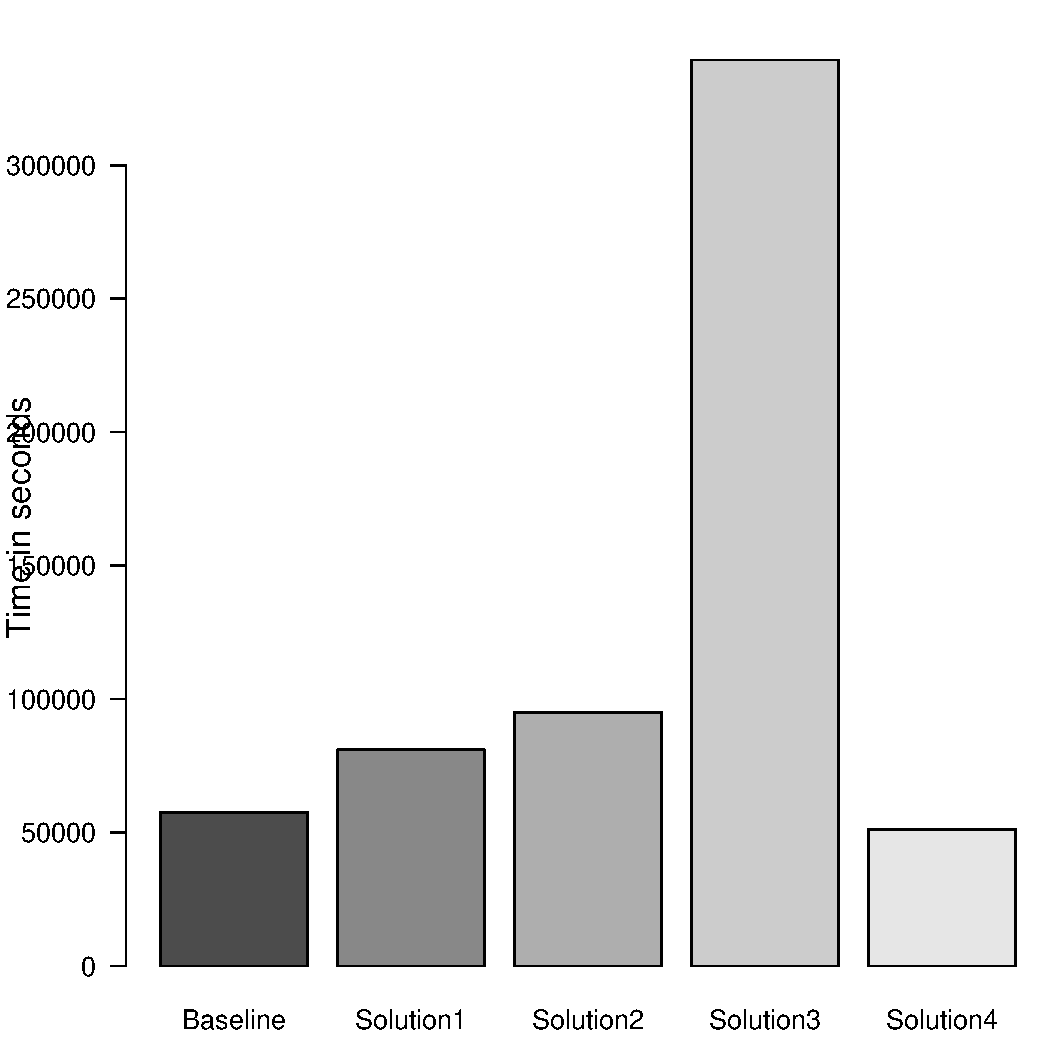
\includegraphics[width=\Width]{figure/result/barplot-insert_student-rt.pdf}}
			\subfigure[Throughput]
			{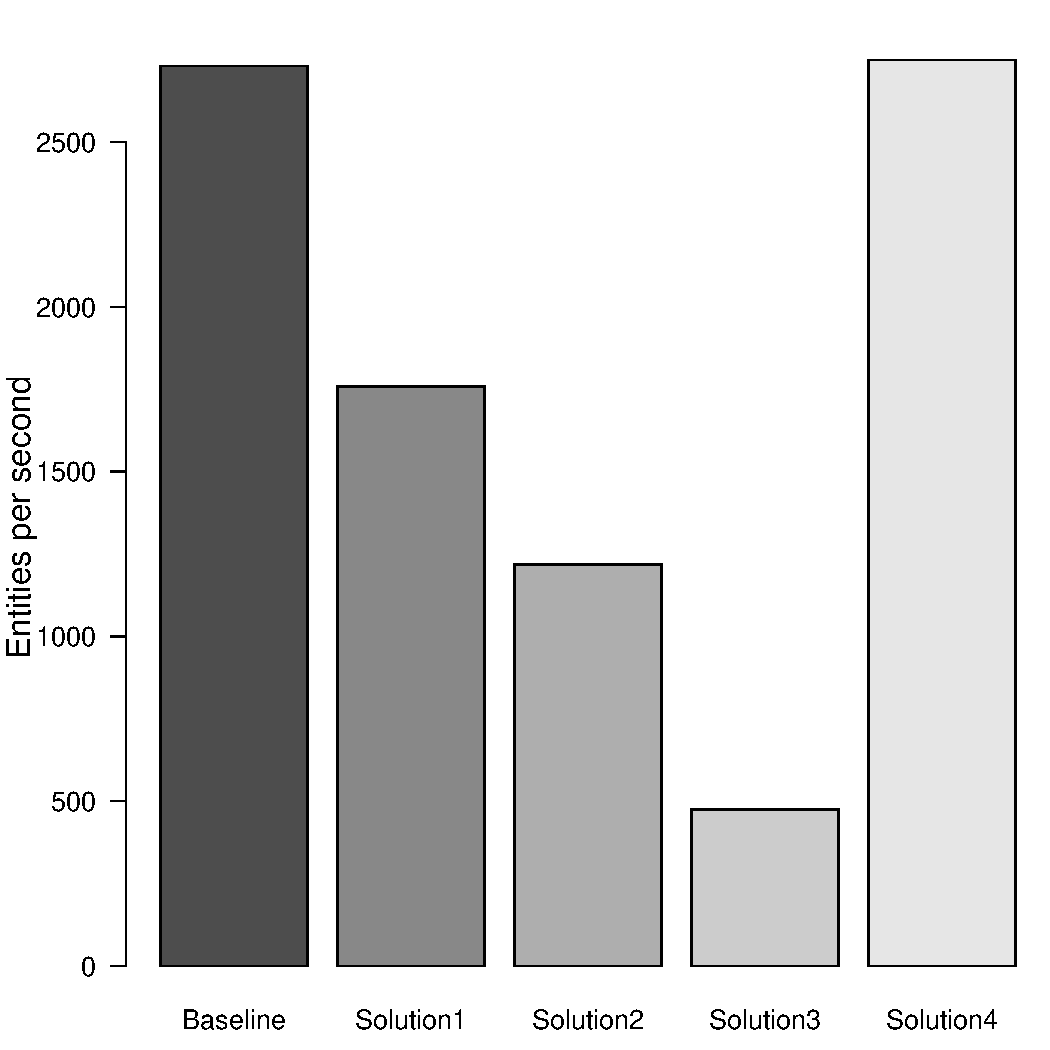
\includegraphics[width=\Width]{figure/result/barplot-insert_student-tp.pdf}}
			\caption{Performance inserting students}\label{f:rd:insert-user}
		\end{figure}
\newpage
	\subsection{Course}
		\begin{figure}[H]
			\subfigure[Response time]
			{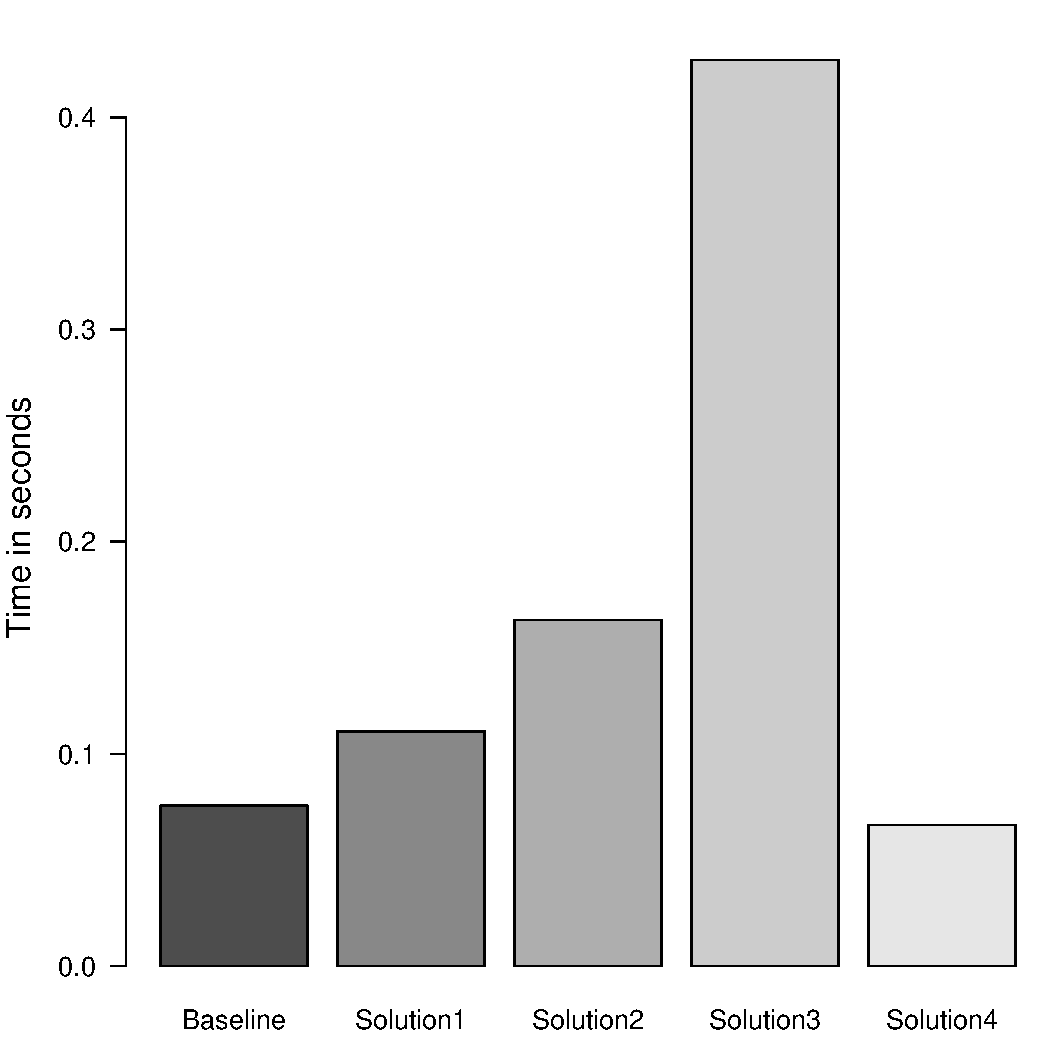
\includegraphics[width=\Width]{figure/result/barplot-insert_course-rt.pdf}}
			\subfigure[Throughput]
			{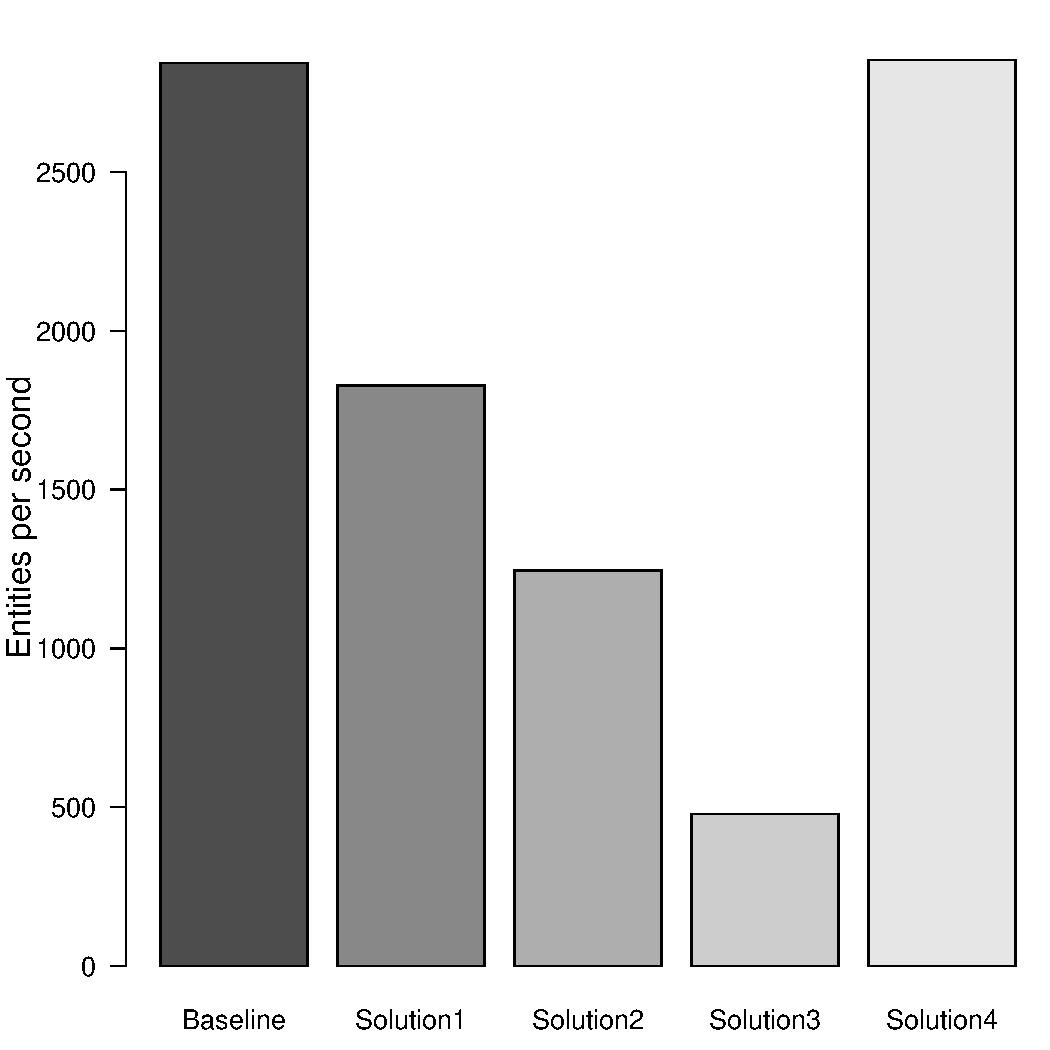
\includegraphics[width=\Width]{figure/result/barplot-insert_course-tp.pdf}}
			\caption{Performance inserting courses}\label{f:rd:insert-course}
		\end{figure}	
\newpage	
	\subsection{Enrolment}
		\begin{figure}[H]
			\subfigure[Response time]
			{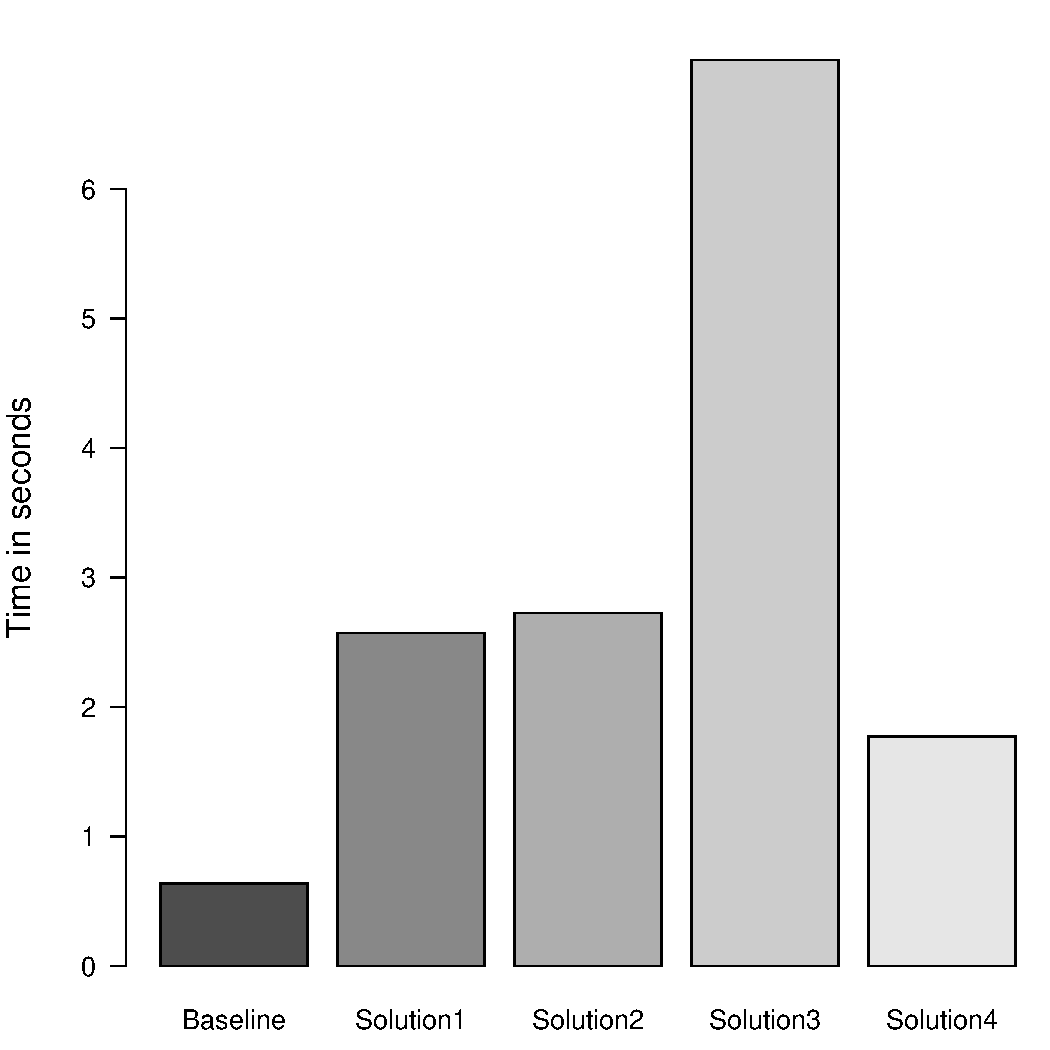
\includegraphics[width=\Width]{figure/result/barplot-insert_enrolment-rt.pdf}}
			\subfigure[Throughput]
			{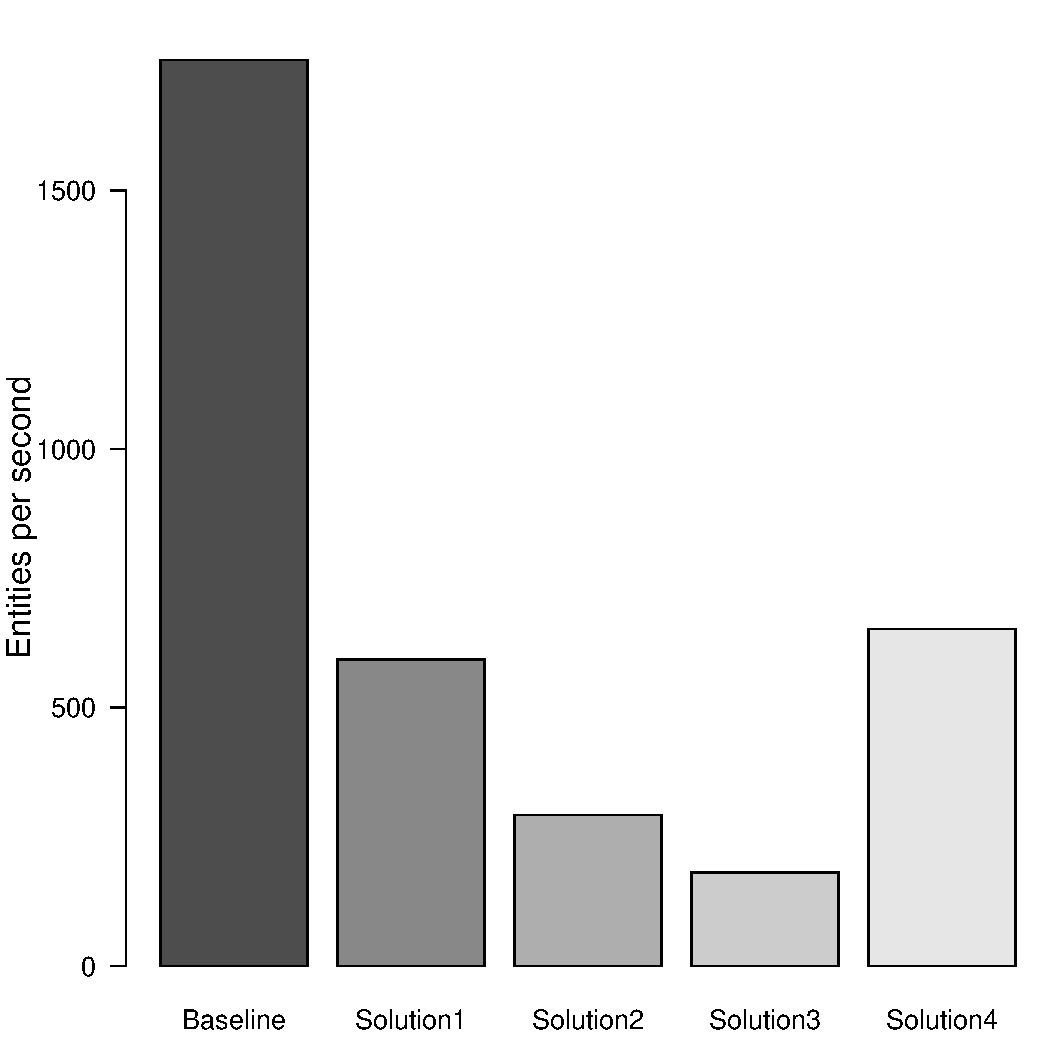
\includegraphics[width=\Width]{figure/result/barplot-insert_enrolment-tp.pdf}}
			\caption{Performance inserting enrolments}\label{f:rd:insert-enrolment}
		\end{figure}
		
\clearpage
\newpage
\section{Update}

	\subsection{Student}
		\begin{figure}[H]
			\subfigure[Response time]
			{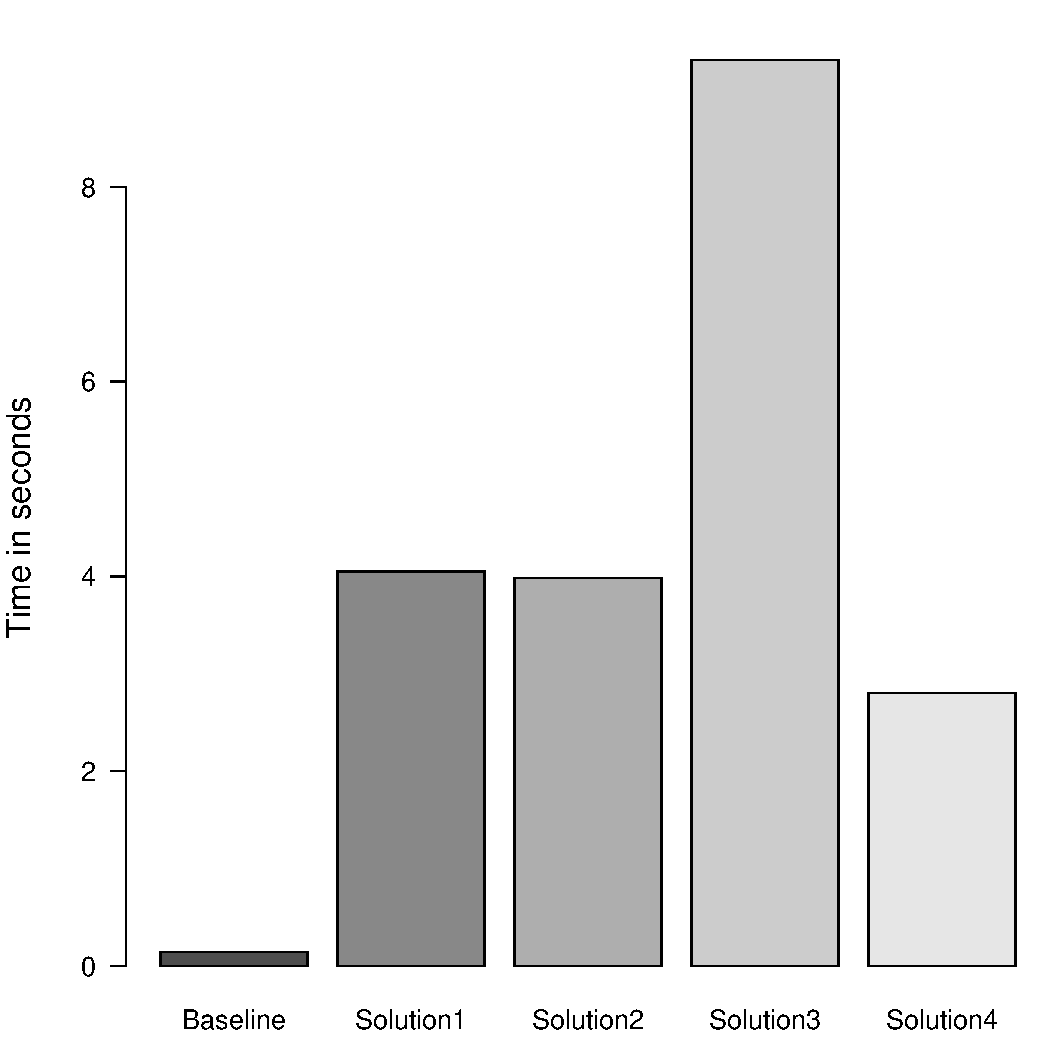
\includegraphics[width=\Width]{figure/result/barplot-update_student-rt.pdf}}
			\subfigure[Throughput]
			{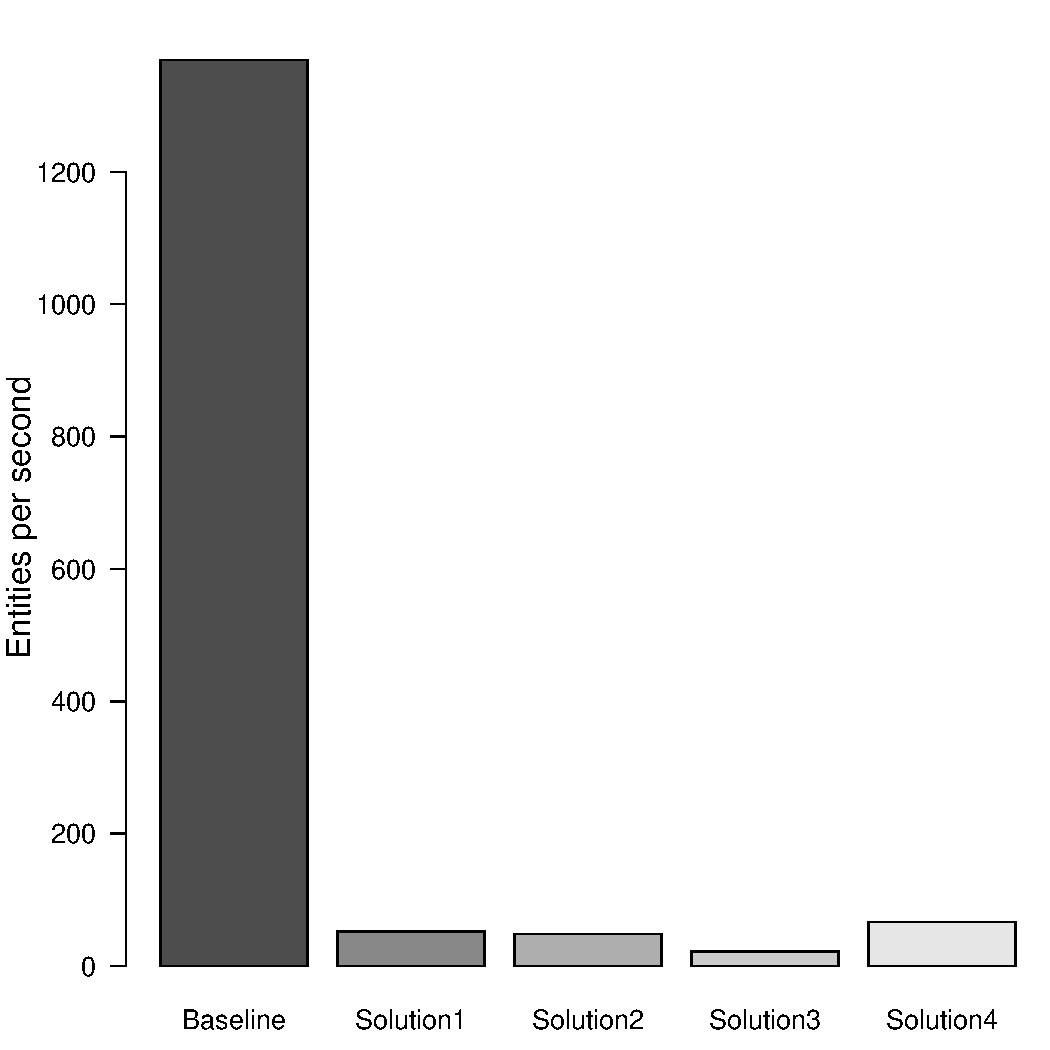
\includegraphics[width=\Width]{figure/result/barplot-update_student-tp.pdf}}
			\caption{Performance updating students}\label{f:rd:update-user}
		\end{figure}
\newpage	
	\subsection{Course} 
		\begin{figure}[H]
			\subfigure[Response time]
			{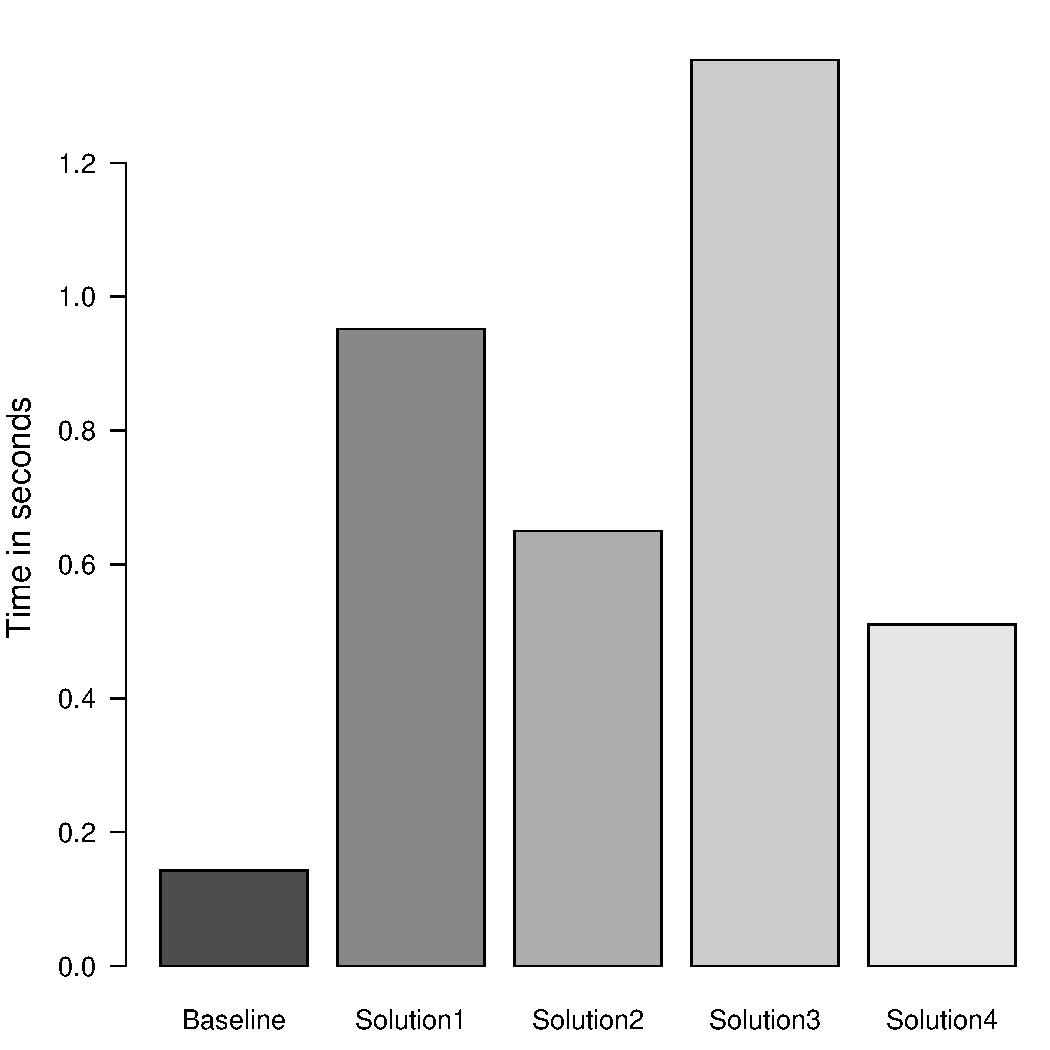
\includegraphics[width=\Width]{figure/result/barplot-update_course-rt.pdf}}
			\subfigure[Throughput]
			{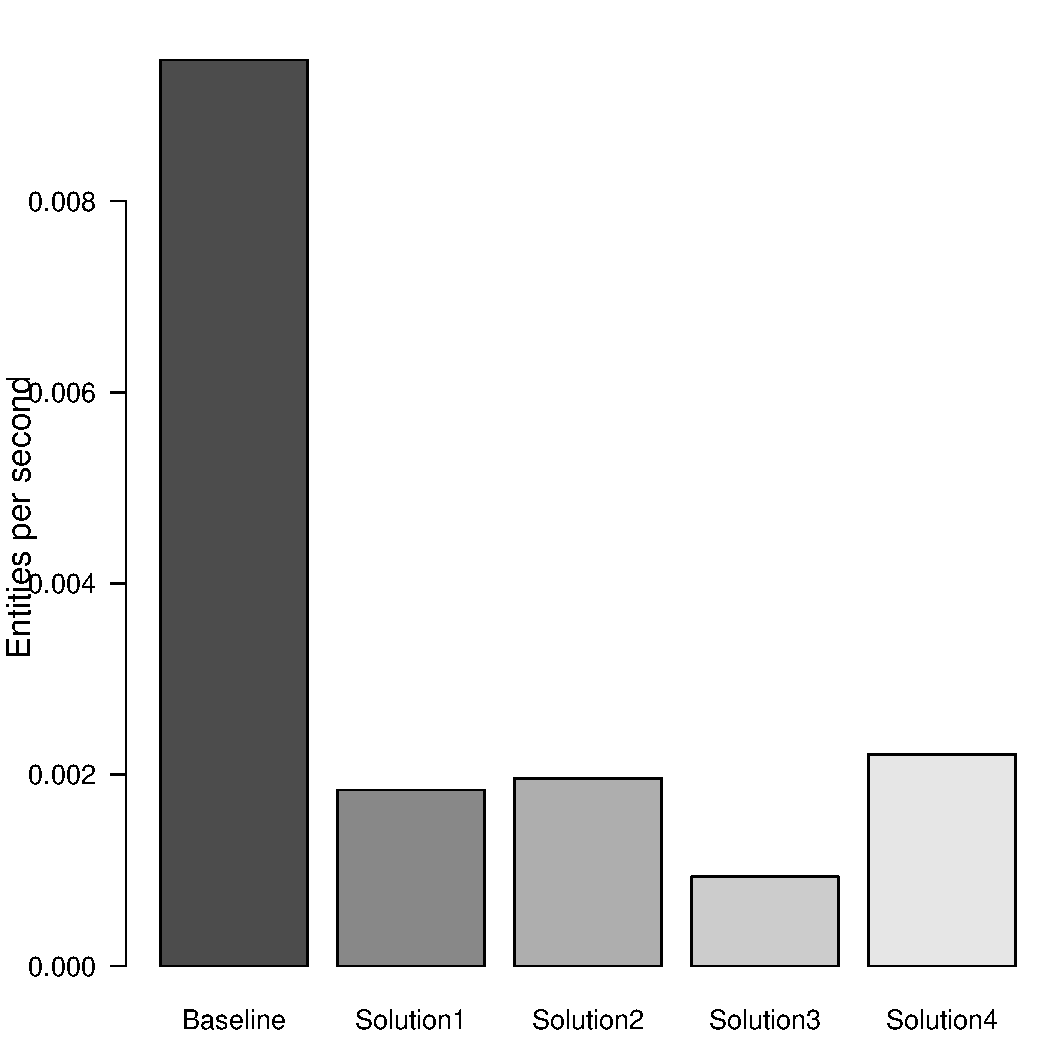
\includegraphics[width=\Width]{figure/result/barplot-update_course-tp.pdf}}
			\caption{Performance updating courses}\label{f:rd:update-course}
		\end{figure}	
\newpage	
	\subsection{Enrolment}
		\begin{figure}[H]
			\subfigure[Response time]
			{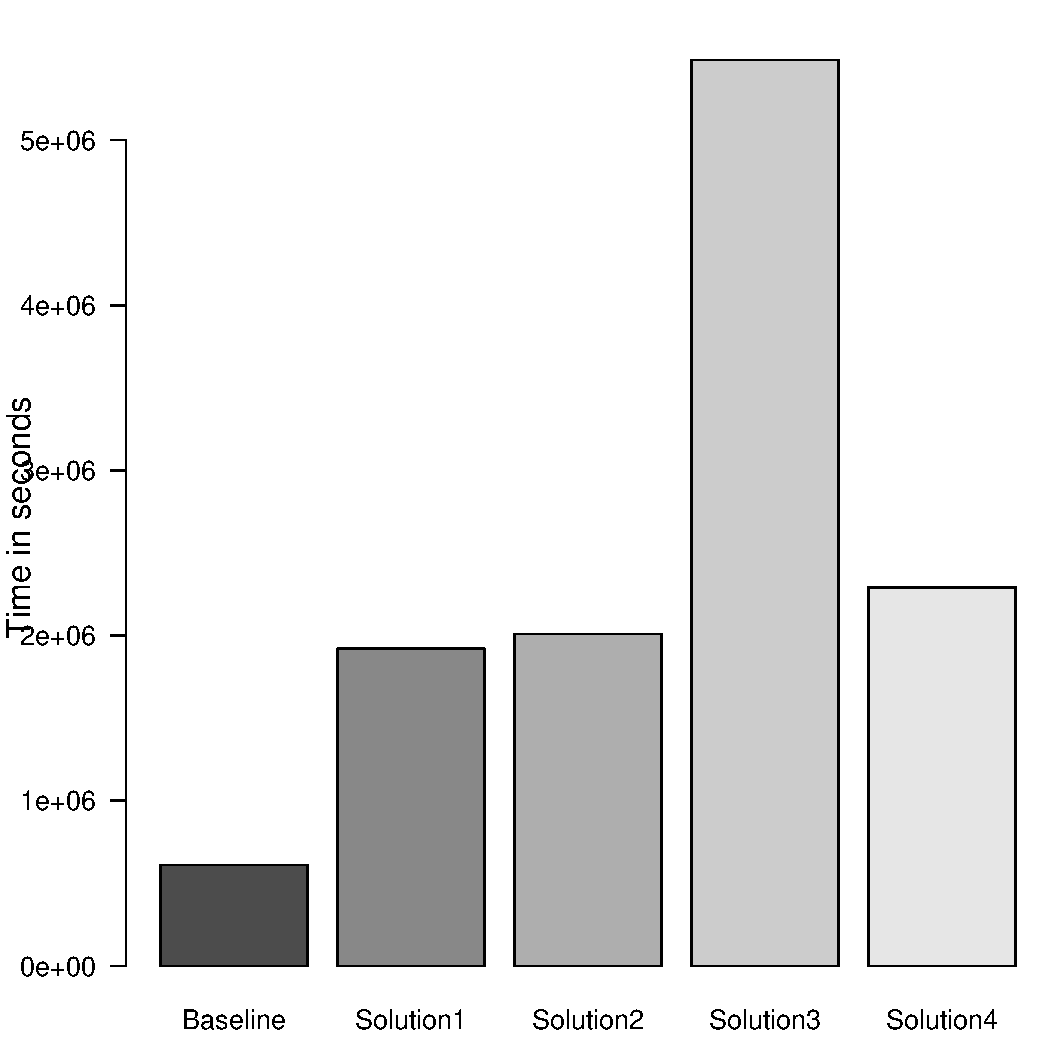
\includegraphics[width=\Width]{figure/result/barplot-update_enrolment-rt.pdf}}
			\subfigure[Throughput]
			{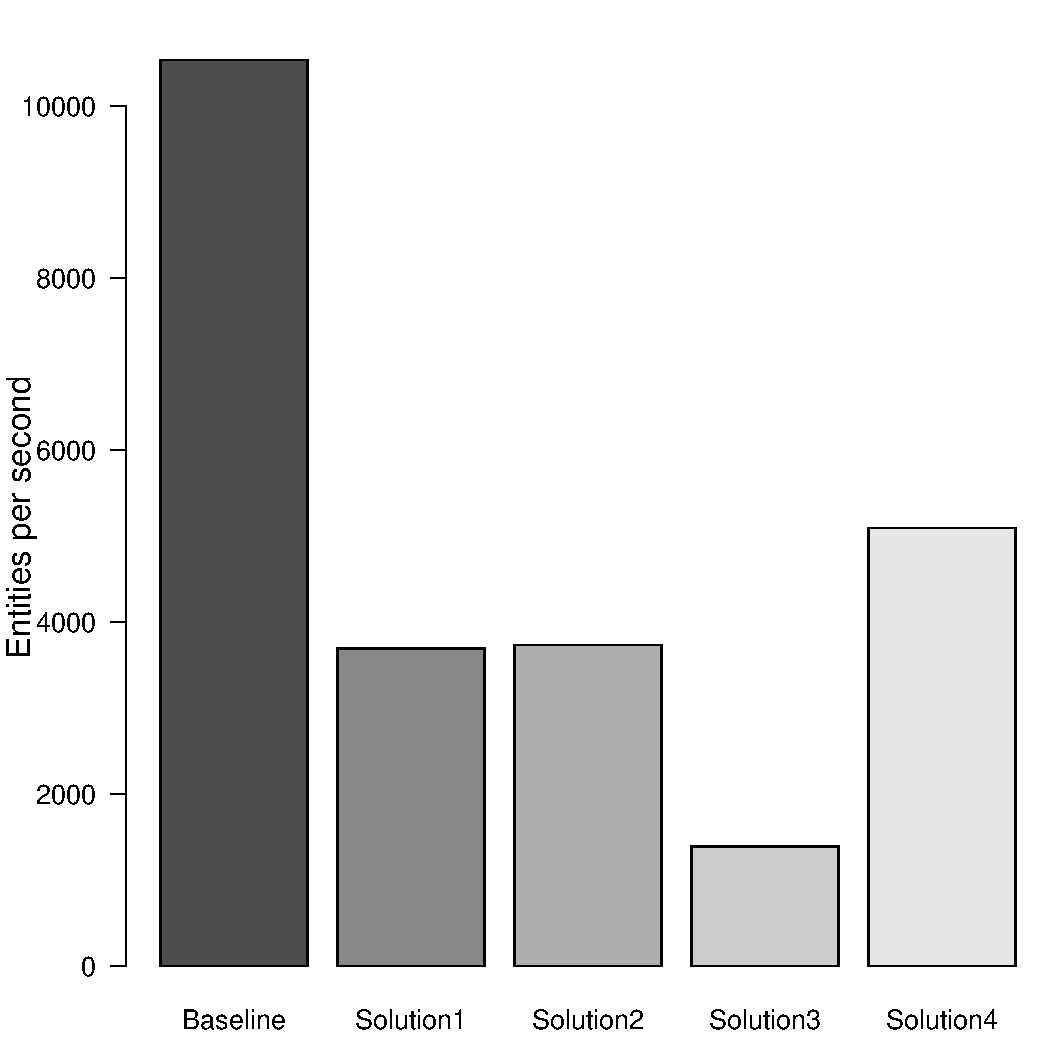
\includegraphics[width=\Width]{figure/result/barplot-update_enrolment-tp.pdf}}
			\caption{Performance updating enrolments}\label{f:rd:update-enrolment}
		\end{figure}
\clearpage
\newpage
\section{Delete} 

	\subsection{Student}
		\begin{figure}[H]
			\subfigure[Response time]
			{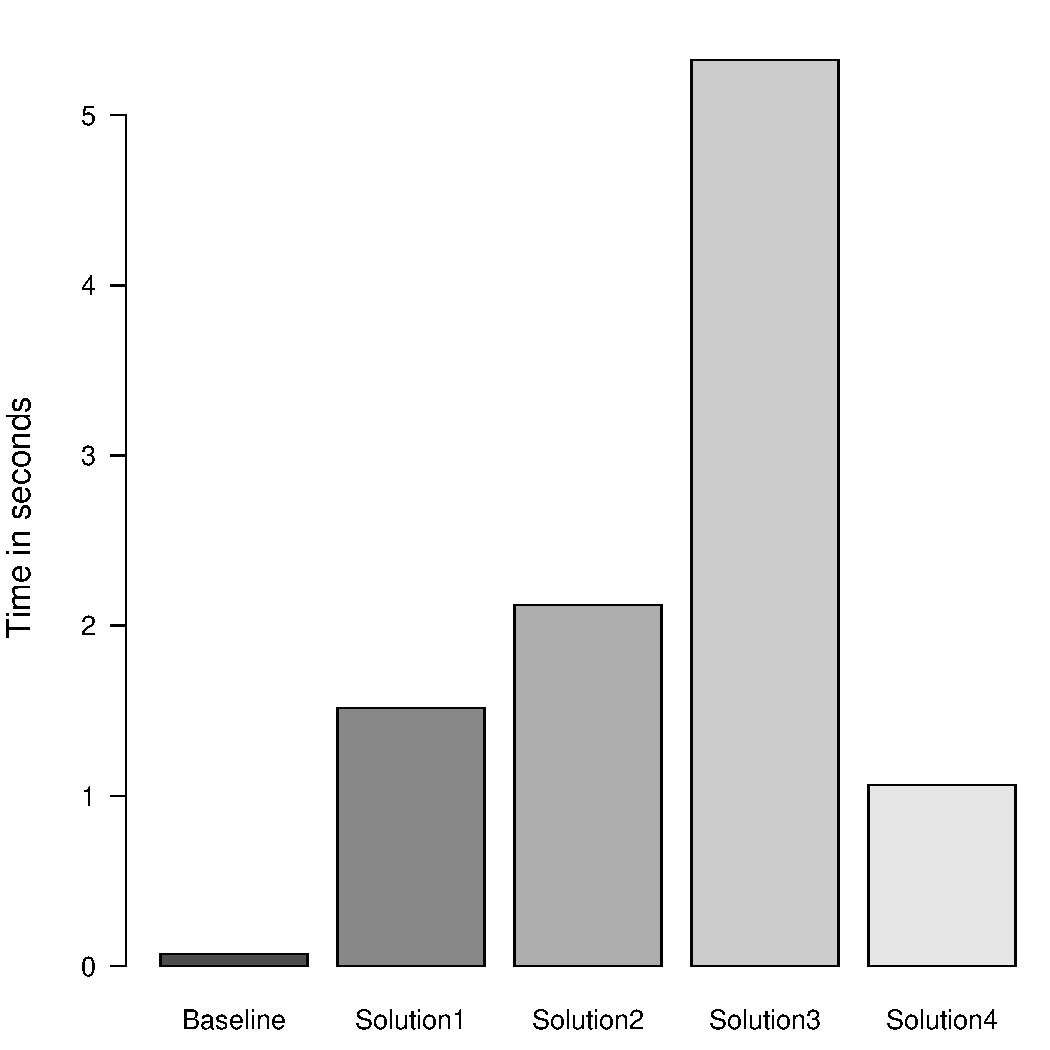
\includegraphics[width=\Width]{figure/result/barplot-delete_student-rt.pdf}}
			\subfigure[Throughput]
			{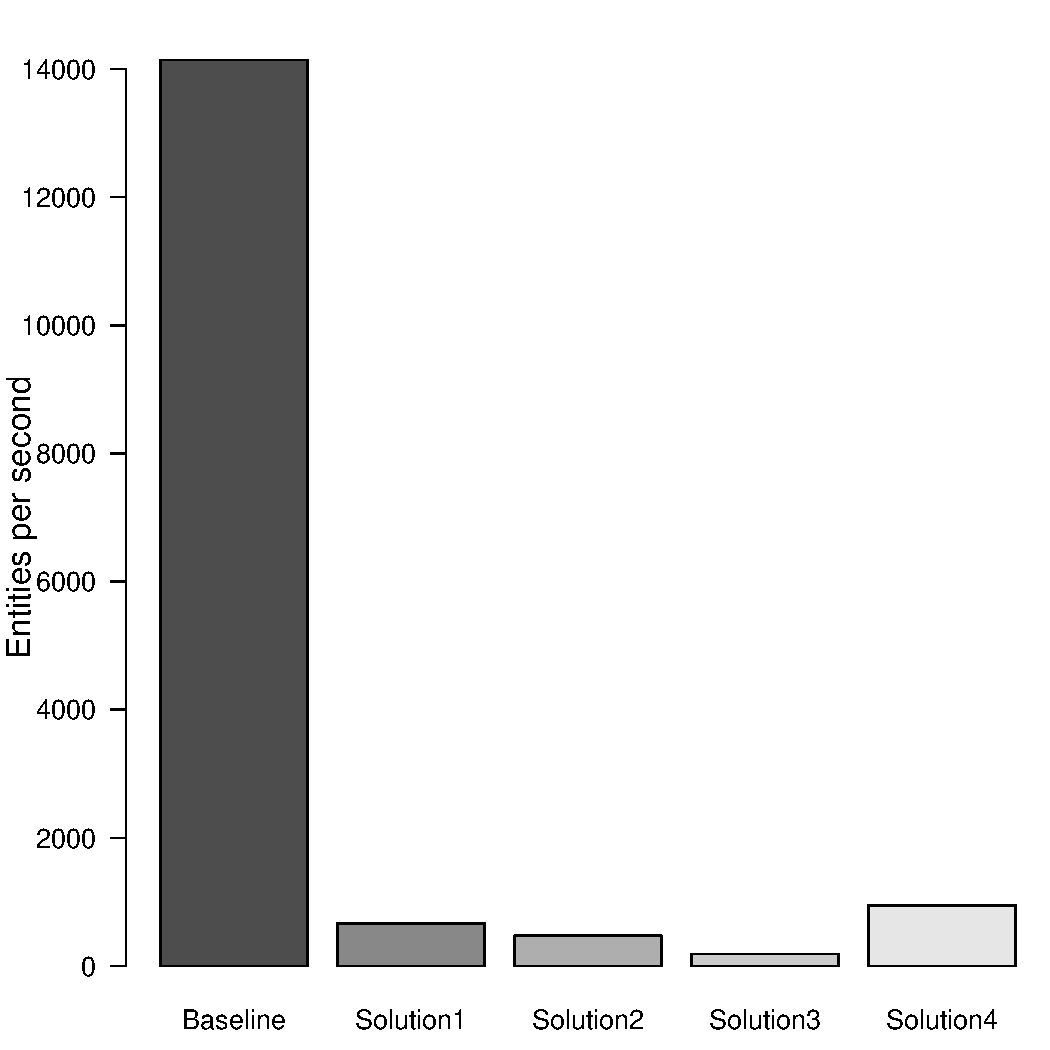
\includegraphics[width=\Width]{figure/result/barplot-delete_student-tp.pdf}}
			\caption{Performance deleting students}\label{f:rd:delete-user}
		\end{figure} 
\newpage	  
	\subsection{Course}
		\begin{figure}[H]
			\subfigure[Response time]
			{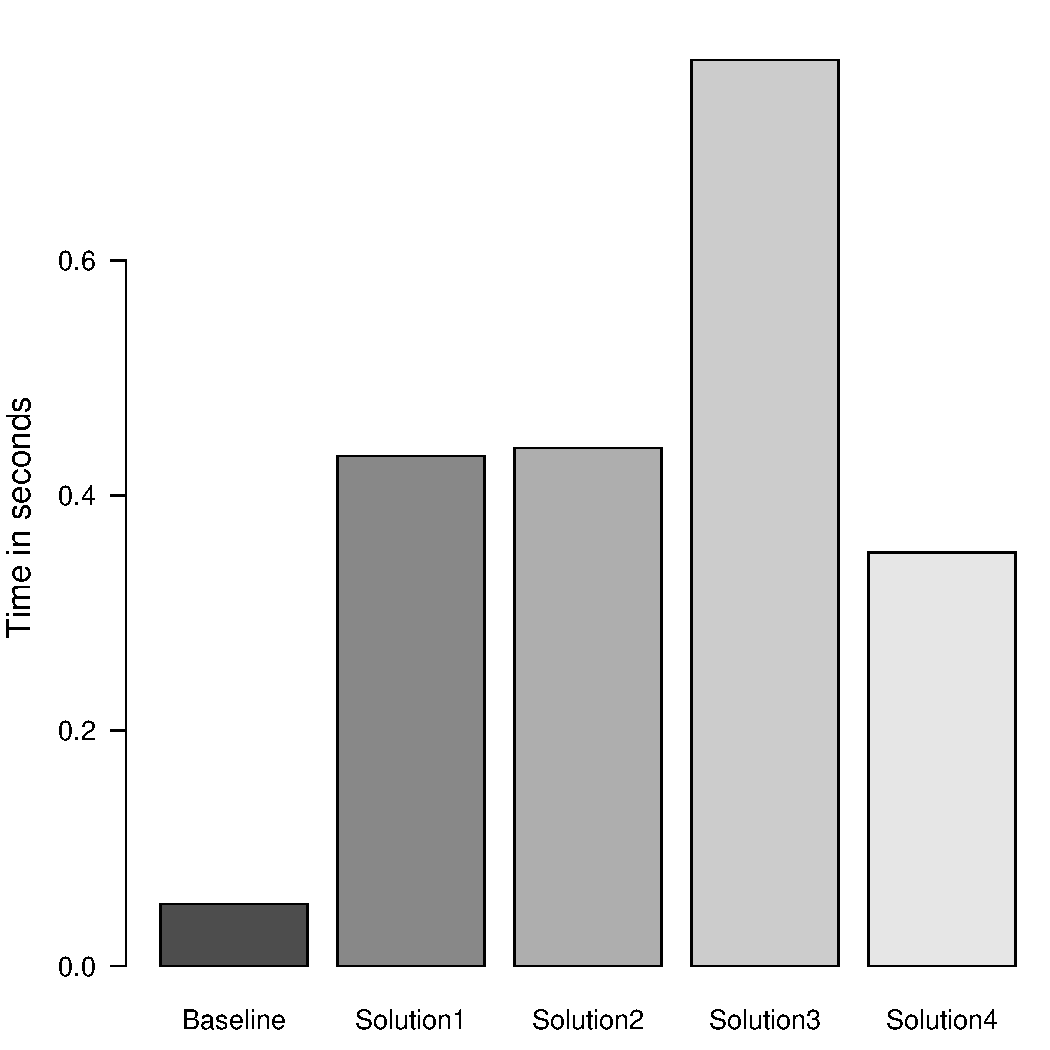
\includegraphics[width=\Width]{figure/result/barplot-delete_course-rt.pdf}}
			\subfigure[Throughput]
			{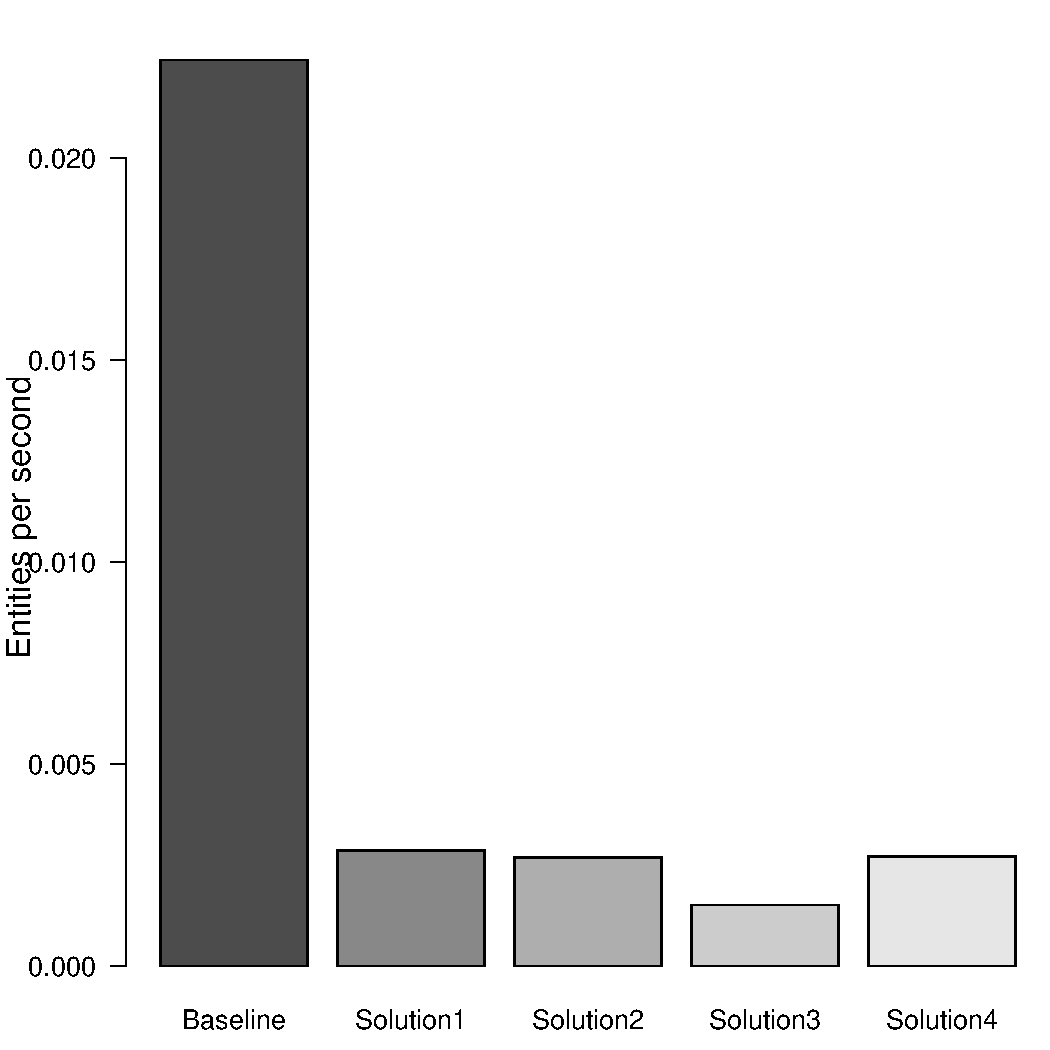
\includegraphics[width=\Width]{figure/result/barplot-delete_course-tp.pdf}}
			\caption{Performance deleting courses}\label{f:rd:delete-course}
		\end{figure}	
\newpage	 
	\subsection{Enrolment}
		\begin{figure}[H]
			\subfigure[Response time]
			{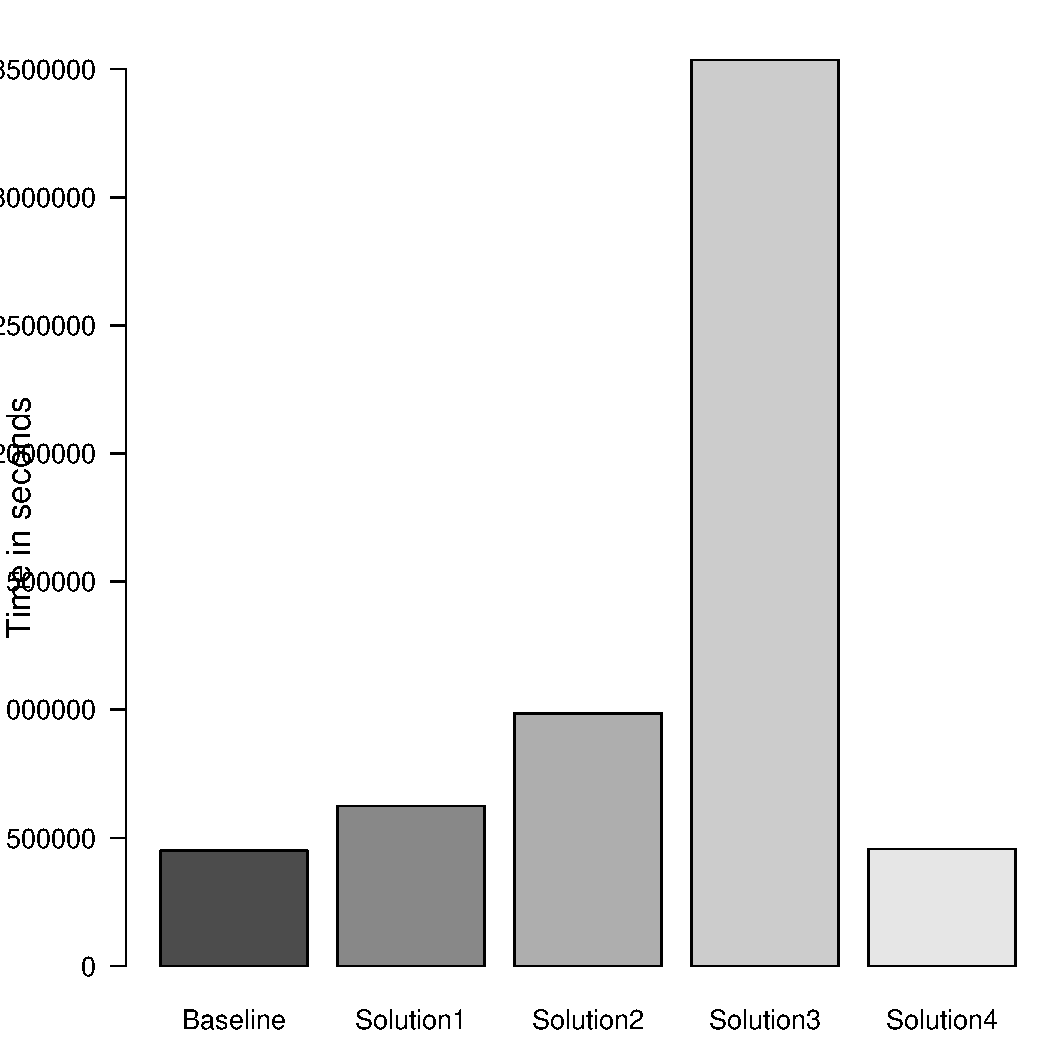
\includegraphics[width=\Width]{figure/result/barplot-delete_enrolment-rt.pdf}}
			\subfigure[Throughput]
			{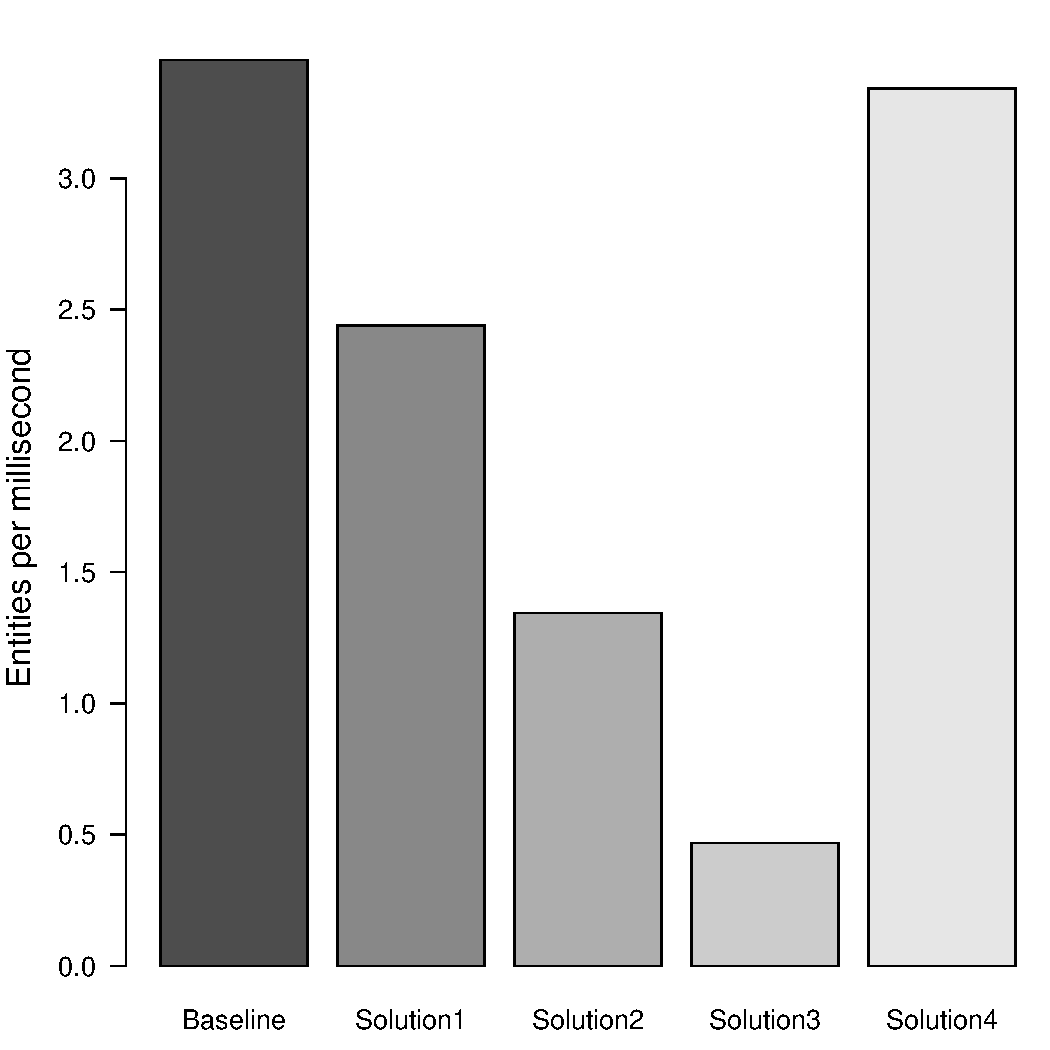
\includegraphics[width=\Width]{figure/result/barplot-delete_enrolment-tp.pdf}}
			\caption{Performance deleting enrolments}\label{f:rd:delete-enrolment}
		\end{figure}
		


	